\documentclass[tikz,border=2mm]{standalone}
\usepackage{polymer-paper-preamble}

\begin{document}
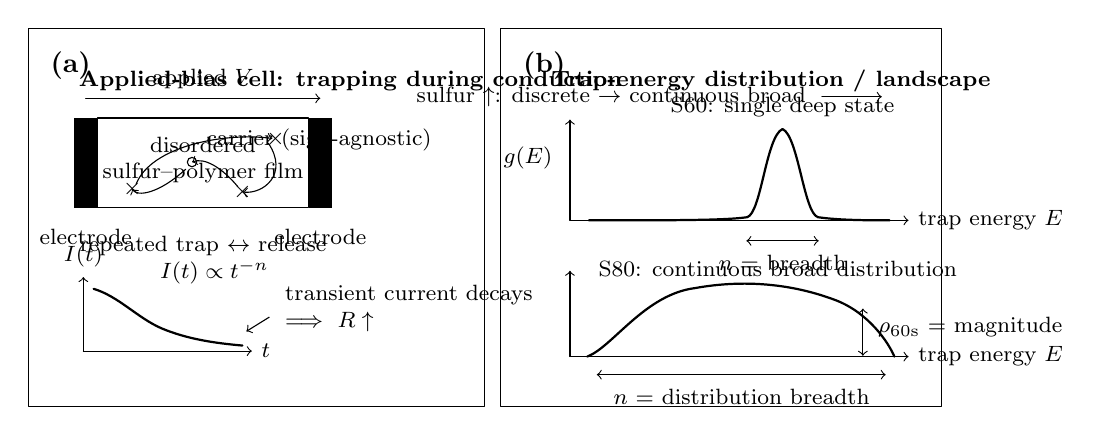
\begin{tikzpicture}[x=1cm,y=1cm,line cap=round,line join=round]
  % Panel frames and labels
  \draw (0,0) rectangle (5.8,4.8);
  \draw (6,0) rectangle (11.6,4.8);
  \node[anchor=north west,font=\bfseries] at (0.16,4.62) {(a)};
  \node[anchor=north west,font=\bfseries] at (6.16,4.62) {(b)};

  % (a) Applied-bias cell and sign-agnostic, repeated trapping.
  \node[anchor=west,font=\footnotesize\bfseries] at (0.52,4.13) {Applied-bias cell: trapping during conduction};
  \fill (0.58,2.52) rectangle (0.88,3.66);
  \fill (3.56,2.52) rectangle (3.86,3.66);
  \draw (0.88,2.52) rectangle (3.56,3.66);
  \node[font=\footnotesize,align=center] at (2.22,3.13) {disordered\\sulfur--polymer film};
  \draw[->] (0.73,3.91) -- (3.71,3.91);
  \node[font=\footnotesize,anchor=south] at (2.22,3.91) {applied $V$};
  \node[font=\footnotesize,anchor=north] at (0.73,2.37) {electrode};
  \node[font=\footnotesize,anchor=north] at (3.71,2.37) {electrode};

  \node[draw,circle,inner sep=1.2pt] (carrier) at (2.08,3.10) {};
  \node[font=\footnotesize,anchor=south west] at (2.14,3.12) {carrier (sign-agnostic)};
  \node[font=\footnotesize] at (1.32,2.76) {$\times$};
  \node[font=\footnotesize] at (2.72,2.72) {$\times$};
  \node[font=\footnotesize] at (3.14,3.40) {$\times$};
  \draw[->] (2.00,3.01) .. controls (1.65,2.69) and (1.38,2.66) .. (1.32,2.76);
  \draw[->] (1.37,2.82) .. controls (1.56,3.30) and (2.48,3.48) .. (3.10,3.40);
  \draw[->] (3.05,3.34) .. controls (3.31,2.95) and (2.99,2.69) .. (2.72,2.72);
  \draw[->] (2.66,2.79) .. controls (2.46,3.03) and (2.24,3.16) .. (2.08,3.10);
  \node[font=\footnotesize,align=center] at (2.22,2.03) {repeated trap $\leftrightarrow$ release};

  % Qualitative CvS decay inset; all labels sit outside the curve.
  \draw[->] (0.70,0.70) -- (2.84,0.70) node[anchor=west,font=\footnotesize] {$t$};
  \draw[->] (0.70,0.70) -- (0.70,1.64) node[anchor=south,font=\footnotesize] {$I(t)$};
  \draw[thick] (0.83,1.49) .. controls (1.14,1.40) and (1.39,1.12) .. (1.69,0.99)
    .. controls (2.02,0.85) and (2.38,0.80) .. (2.72,0.77);
  \node[anchor=south west,font=\footnotesize] at (1.55,1.43) {$I(t)\propto t^{-n}$};
  \node[anchor=west,font=\footnotesize,align=left] at (3.14,1.24) {transient current decays\\$\Longrightarrow\ R\uparrow$};
  \draw[->] (3.06,1.13) -- (2.77,0.95);

  % (b) Composition-dependent trap-energy distributions.
  \node[anchor=west,font=\footnotesize\bfseries] at (6.52,4.13) {Trap-energy distribution / landscape};
  \node[font=\footnotesize,anchor=east] at (6.78,3.15) {$g(E)$};
  \draw[->] (6.88,2.36) -- (11.18,2.36) node[anchor=west,font=\footnotesize] {trap energy $E$};
  \draw[->] (6.88,2.36) -- (6.88,3.64);

  % S60: one narrow peak at the deep-energy side.
  \draw[thick] (7.12,2.36) .. controls (8.22,2.36) and (8.85,2.36) .. (9.13,2.40)
    .. controls (9.31,2.45) and (9.37,3.43) .. (9.58,3.52)
    .. controls (9.78,3.43) and (9.85,2.45) .. (10.03,2.40)
    .. controls (10.30,2.36) and (10.71,2.36) .. (10.94,2.36);
  \node[font=\footnotesize,anchor=south] at (9.58,3.55) {S60: single deep state};
  \draw[<->] (9.12,2.10) -- (10.04,2.10);
  \node[font=\footnotesize,anchor=north] at (9.58,2.04) {$n$ = breadth};

  % S80: continuous, broad distribution, with magnitude orthogonal to breadth.
  \draw[->] (6.88,0.63) -- (11.18,0.63) node[anchor=west,font=\footnotesize] {trap energy $E$};
  \draw[->] (6.88,0.63) -- (6.88,1.72);
  \draw[thick] (7.10,0.63) .. controls (7.42,0.75) and (7.83,1.42) .. (8.47,1.50)
    .. controls (9.08,1.61) and (9.70,1.56) .. (10.27,1.34)
    .. controls (10.67,1.18) and (10.92,0.82) .. (11.00,0.63);
  \node[font=\footnotesize,anchor=west] at (7.12,1.74) {S80: continuous broad distribution};
  \draw[<->] (7.22,0.40) -- (10.89,0.40);
  \node[font=\footnotesize,anchor=north] at (9.06,0.34) {$n$ = distribution breadth};
  \draw[<->] (10.60,0.64) -- (10.60,1.24);
  \node[font=\footnotesize,anchor=west] at (10.67,1.00) {$\rho_{60\mathrm{s}}$ = magnitude};

  \draw[->] (10.08,3.93) -- (10.84,3.93);
  \node[font=\footnotesize,anchor=east] at (10.00,3.93) {sulfur $\uparrow$: discrete $\rightarrow$ continuous broad};
\end{tikzpicture}
\end{document}
